\section{System Architecture}

A general concern when designing large systems is the accidental
complexity\cite[p.~8-9]{holt2004uml} one may create by making poor design choices early
on. Many solutions designed to reduce accidental complexity are based around
software systems, and sacrifices performance in the domains of both time and
space\cite{moseley2006out}. While these solutions may be applicable
within hardware systems where these kinds of performance degradations are not a
problem, it is unacceptable in systems where one or multiple of the system
requirements are a performance increase in one or both of these domains. As one
of our main requirements is focus on performance, we have to accept a certain
level of inherent complexity.
\begin{figure}[h]
  \centering
  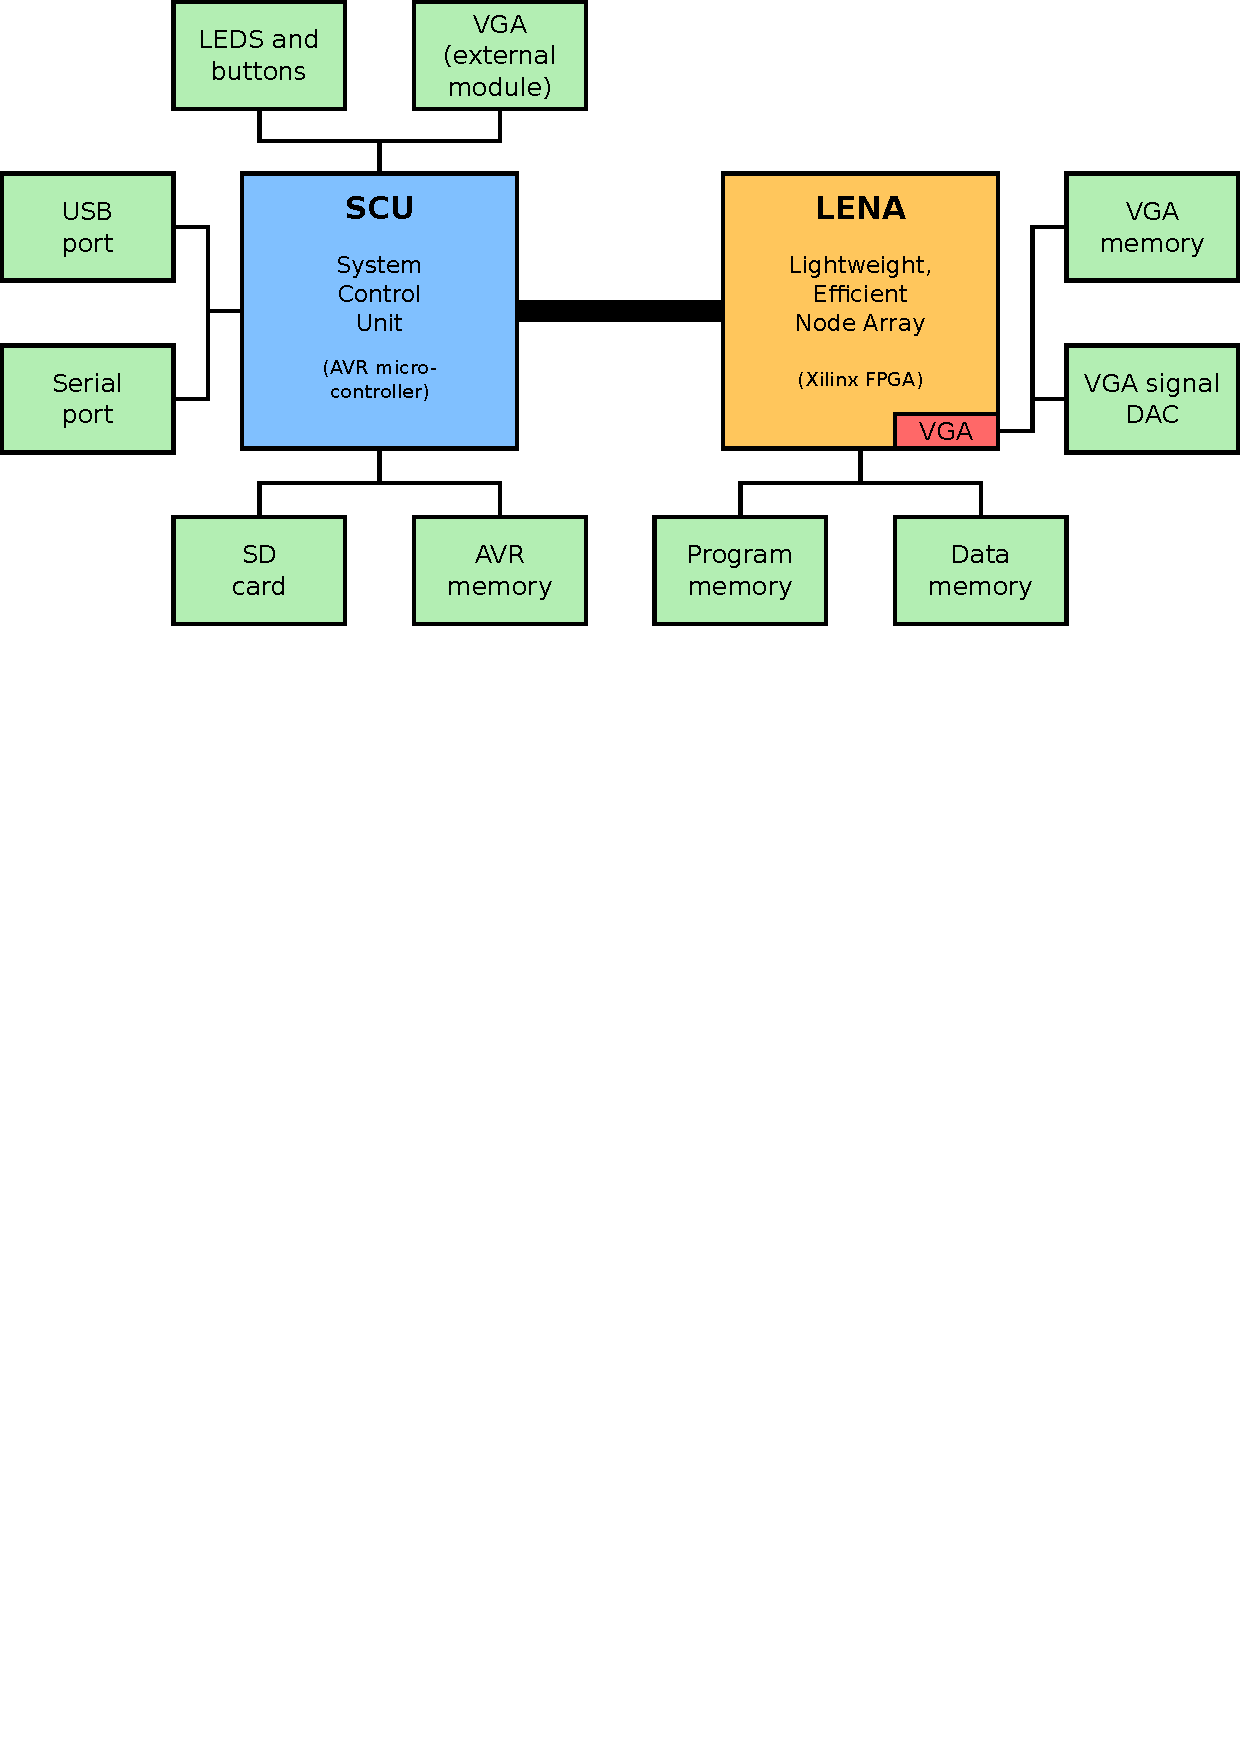
\includegraphics[width=\linewidth,clip,trim=0 18cm 0 0]
                  {fig/sys-over/arch-fig.pdf}
  \caption{System Architecture}
  \label{fig:sys-over-arch-fig}
\end{figure}


To remedy the complexity which inevitably follows from our requirements, we
focused on making it possible to both isolate errors and test
individual components as early as possible: The \ac{LENA} architecture was
tested through \ac{VHDL} test benches, the \ac{VGA} component was tested with
prototypes on a breadboard, and the \ac{SCU} was tested with an EVK1100 development
board as well as with the buttons and \ac{LED}s on the PCB once it arrived.
By doing this, we could assume that errors occurring when connecting different
components are mostly due to errors in the protocol implementation(s).

Figure \ref{fig:sys-over-arch-fig} shows our resulting architecture. We also included a
\ac{VGA} connector connected to the AVR, in case the \ac{LENA} architecture
should fail to implement its \ac{VGA} module.

To be able to process data, we needed an \ac{I/O} device which could serve the machine
with data it should process. To ensure that we would have at least one
functional \ac{I/O} component, we included both a serial
port, a \ac{USB} port and an \ac{SD} card reader on the \ac{PCB}. In addition,
to be able to keep enough data in memory and allow full overlap of different memory
transactions to make processing fast, the \ac{LENA} architecture has three separate
memory components. One for \ac{VGA}, one for instructions and one for data.
